\documentclass[10pt]{article}
%%%%%%%%%%%%%
%windows 正常 ok
\usepackage{ctex} % 加载中文支持宏包
%macos ok
%\usepackage{fontspec}
%\usepackage{xeCJK}  % 如果你需要支持中文
%%%%%%%%%%%%%

\usepackage[x11names]{xcolor} % 启用更多颜色选项
\usepackage{amsmath}      % 数学公式
\usepackage{graphicx}     % 图片插入
\usepackage{rotating} % 引入rotating包
\usepackage{pdfpages}
\usepackage{listings}     % 用于插入代码
\usepackage{hyperref}     % 超链接支持
\usepackage{geometry}     % 设置页边距
\usepackage{fancyhdr}     % 页眉页脚设置
\usepackage{multicol}   % 多栏排版
\usepackage{tocbibind}    % 目录、参考文献包含在目录中
\geometry{a4paper, left=0.6in, right=0.5in, top=0.5in, bottom=0.5in}

% 设置列表中Java代码的样式
\lstdefinestyle{java}{
    language=Java,
%    backgroundcolor=\color{lightgray}, % 背景颜色
    basicstyle=\ttfamily\footnotesize, % 字体
    breaklines=true,                   % 自动换行
    captionpos=b,                      % 标题位置
%    numbers=left,                      % 行号位置
%    numberstyle=\tiny\color{gray},     % 行号样式
    keywordstyle=\color{blue},         % 关键词颜色
    stringstyle=\color{red},           % 字符串颜色
    commentstyle=\color{green},        % 注释颜色
%    frame=single                       % 边框
}

% 设置页眉和页脚
\pagestyle{fancy}
\fancyhf{}
\fancyhead[L]{技术学习} % 左边页眉
\fancyhead[C]{sully} % 中间页眉
\fancyhead[R]{202501} % 右边页眉
\fancyfoot[C]{\thepage} % 页脚中间显示页码

\title{技术学习}
\author{sully}
\date{\today}

\begin{document}

\maketitle

% 生成目录
\tableofcontents
\newpage

\section{引言}
这里是文章的引言部分。

\section{Java代码示例}
以下是一个嵌入的Java代码示例:

\begin{lstlisting}[style=java, caption={HelloWorld.java}]
public class HelloWorld {
    public static void main(String[] args) {
        System.out.println("Hello, world!");
    }
}
\end{lstlisting}

\section{图片插入示例}
下面是一个插入图片的示例:

\begin{figure}[h]
    \centering
    
\includegraphics[width=0.5\textwidth]{9.png} % 确保替换为你的图片路径
    \caption{示例图片}
    \label{fig:example}
\end{figure}

\newpage
\section{引言}
这里是文章的引言部分。

\newpage
\section{插入C++代码}
%\lstinputlisting[language=java]{Hello.java}
%\input{Hello.txt}
%\usepackage{verbatim}
%\verbatiminput{Hello.txt}

本文展示了如何嵌入Java代码和图片,同时提供了目录、章节标题等结构。


\newpage
\section{简历样本与我的简历}
\begin{figure}[h]
  \centering
  \begin{sideways} %选择图片
    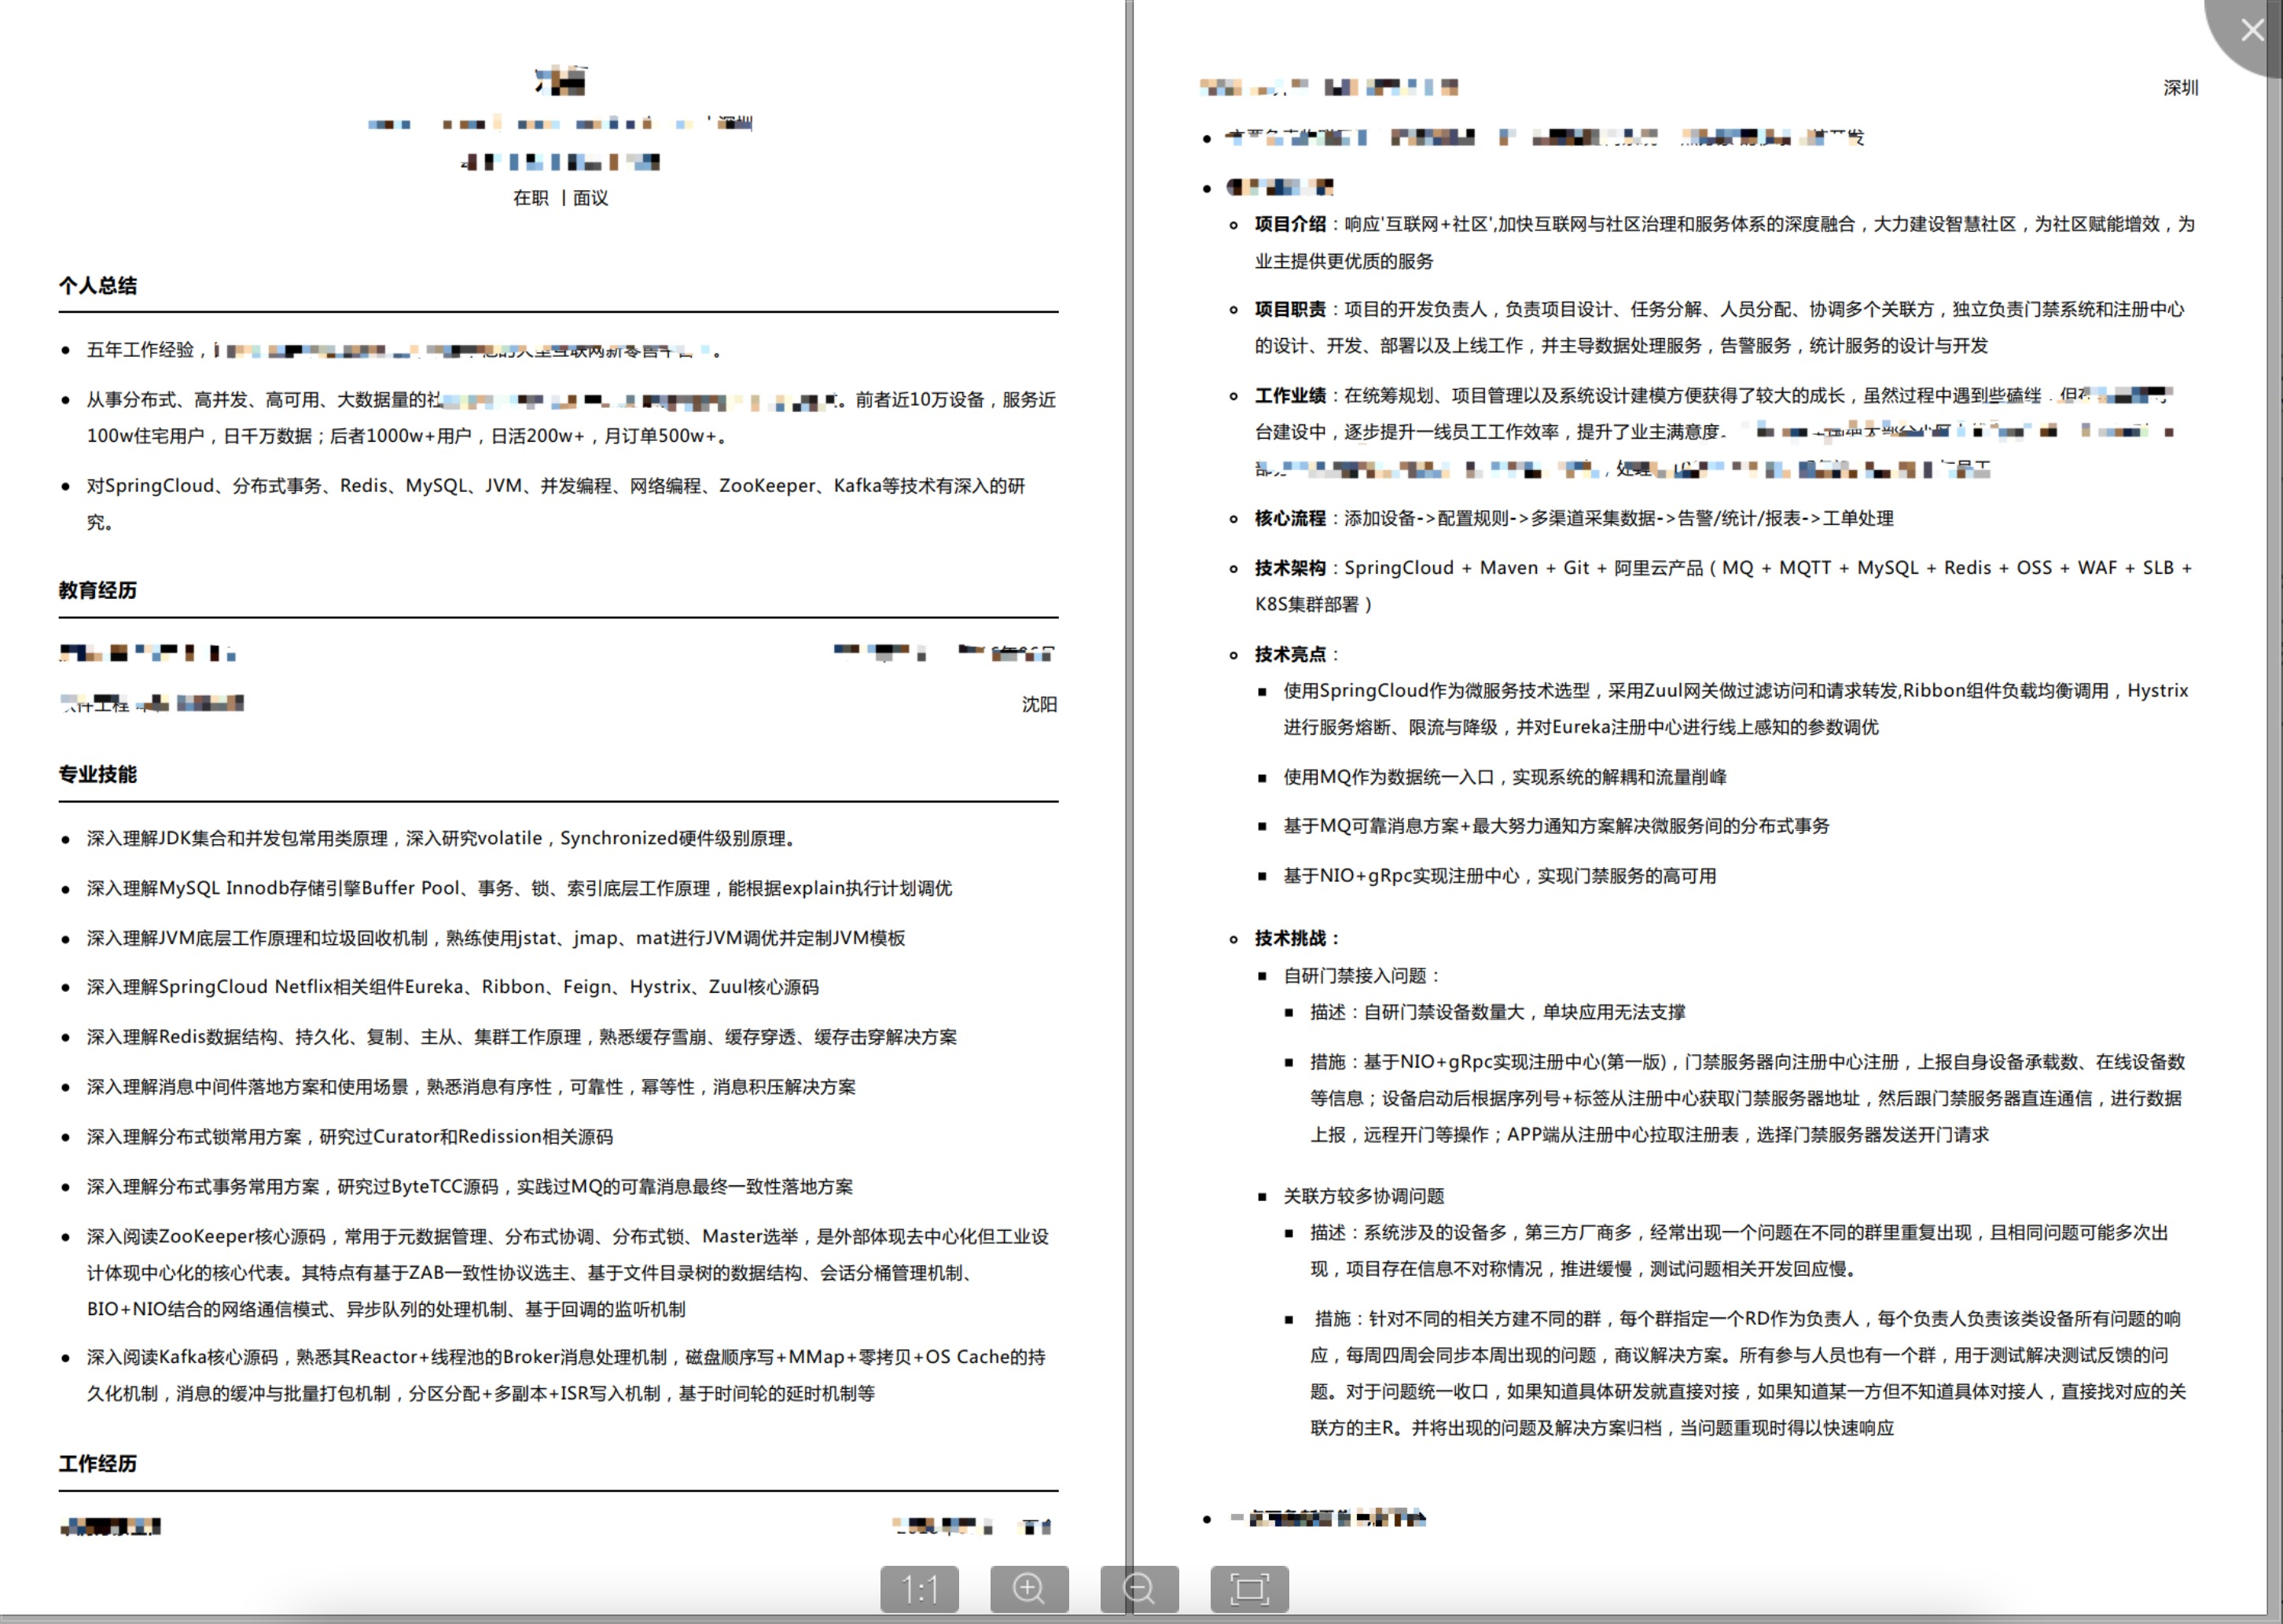
\includegraphics[width=1.0\textwidth]{resumes_ample.jpg} % 确保替换为你的图片路径
    %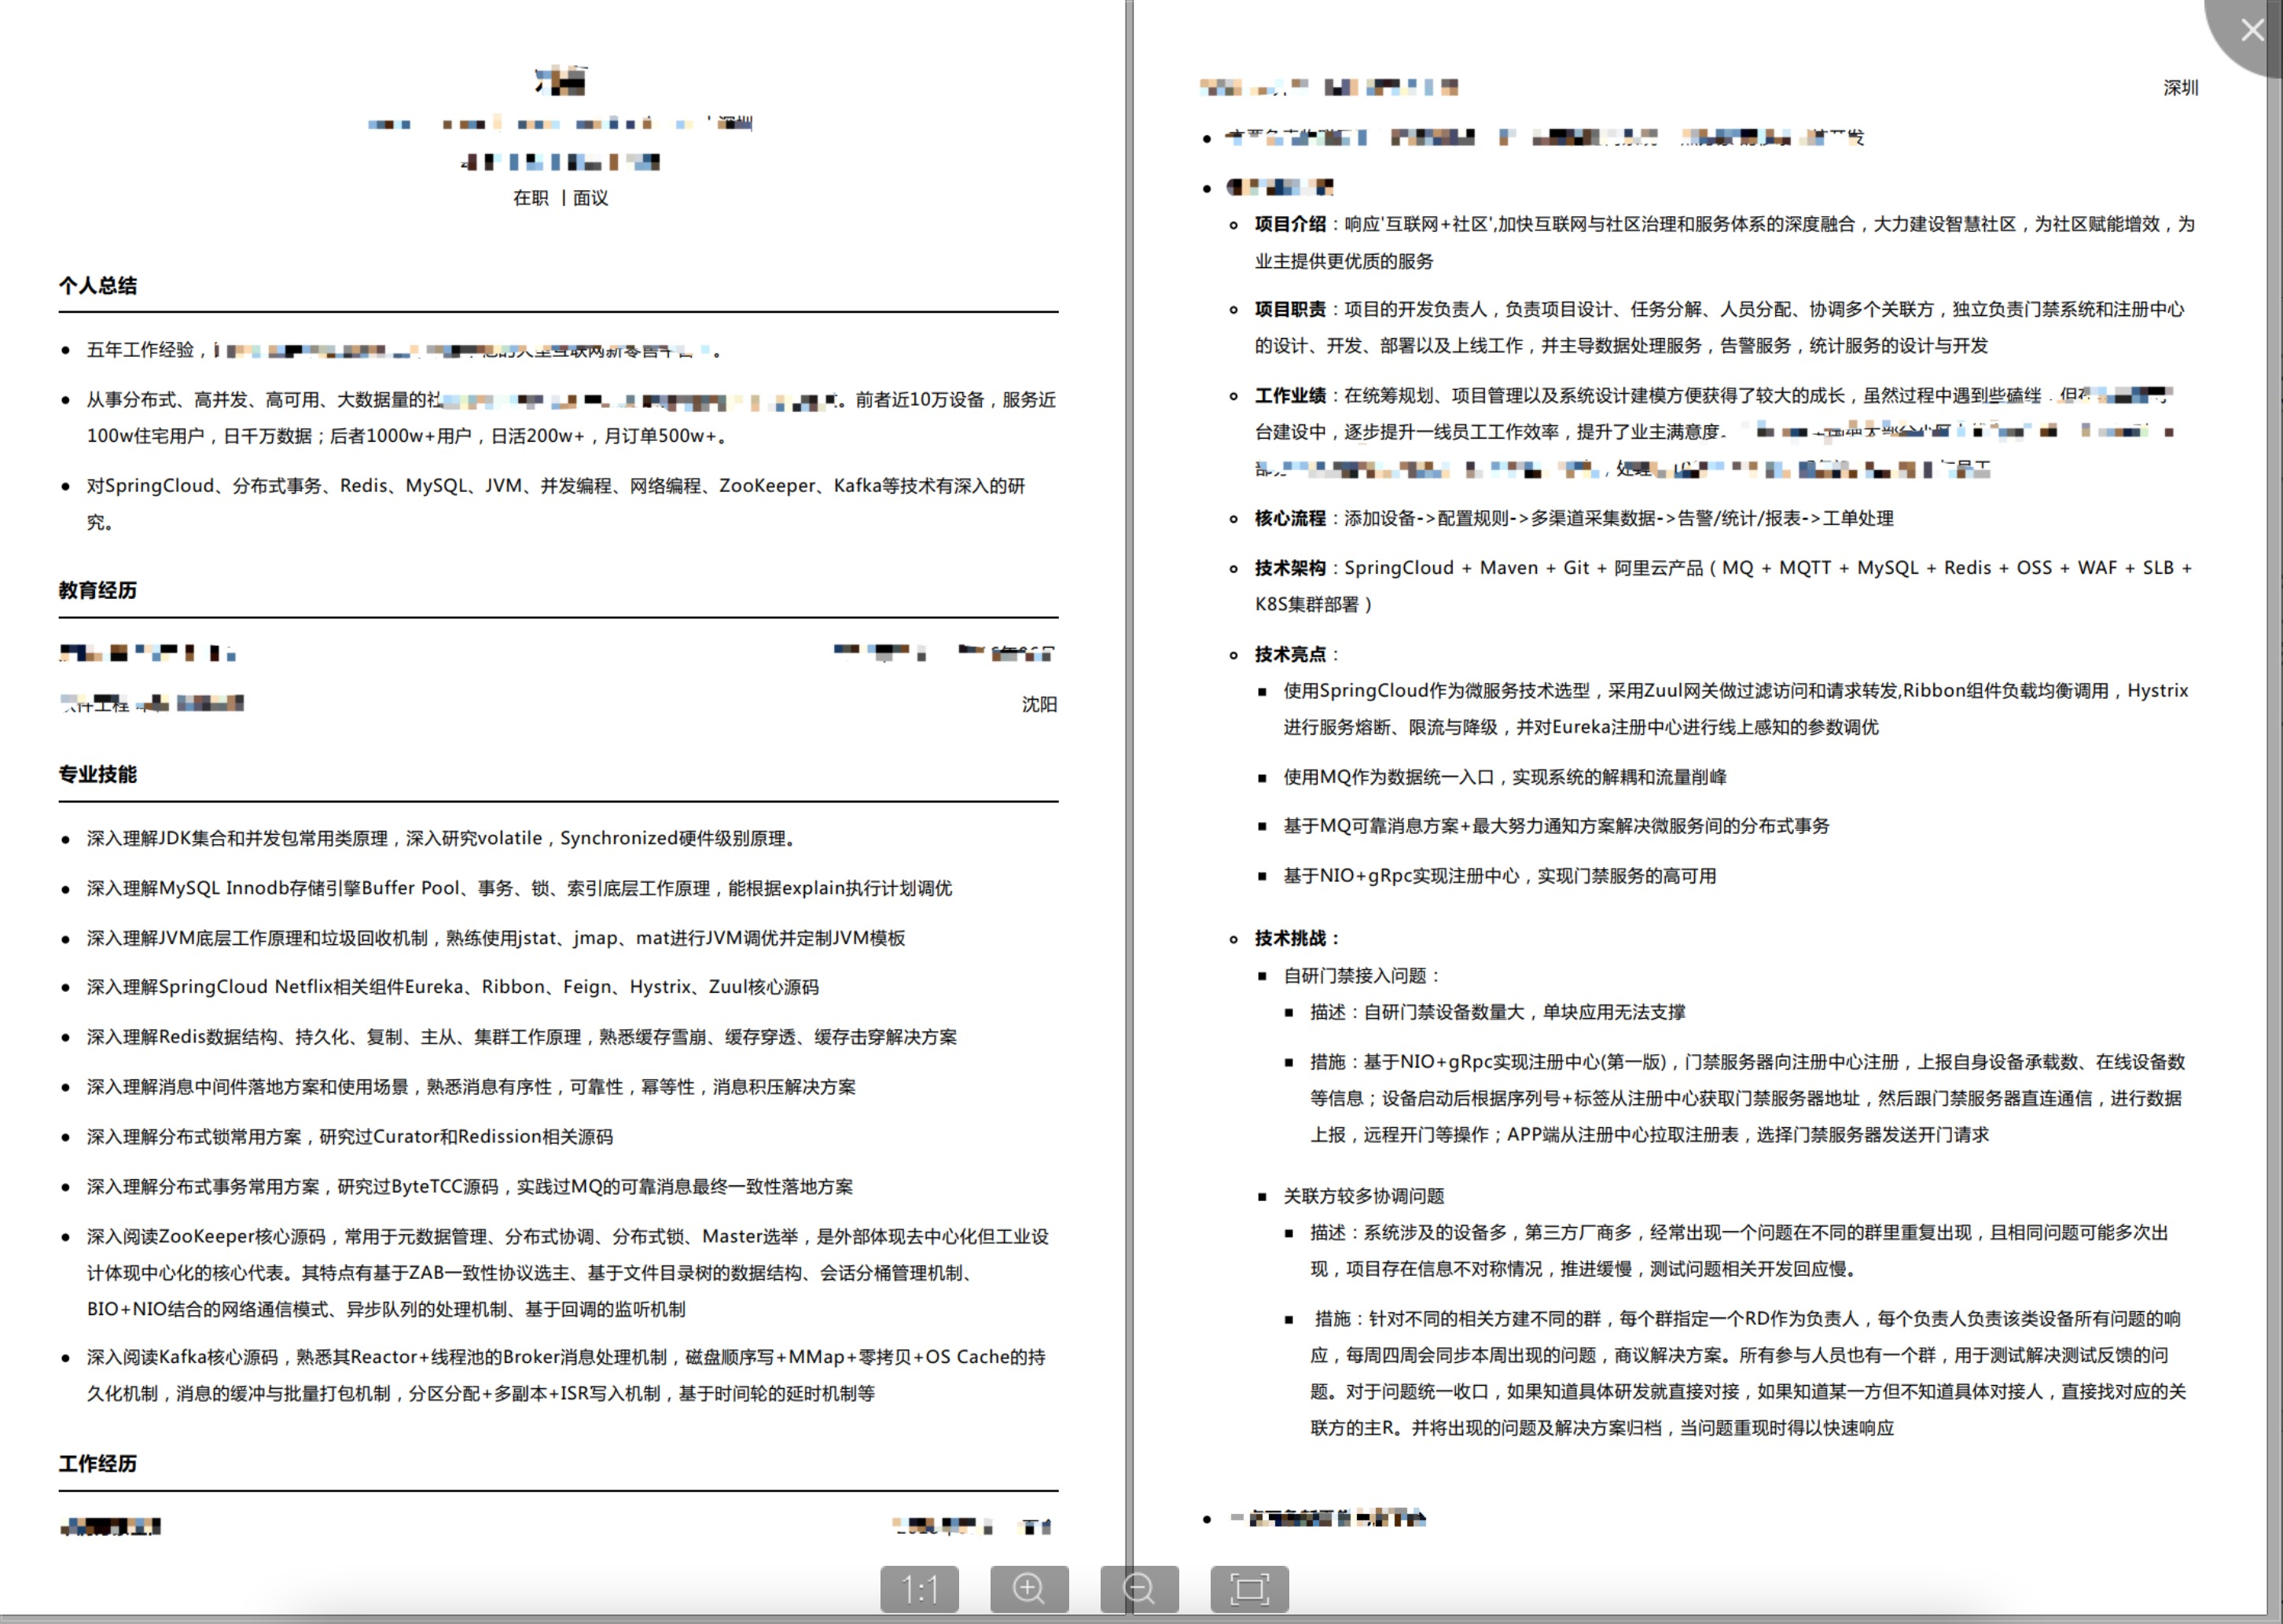
\includegraphics[width=\textwidth, height=\textheight]{resumes_ample.jpg} % 确保替换为你的图片路径    
  \end{sideways}
    \caption{简历样本}
    \label{fig:example}
  \end{figure}



\newpage
%\section{我的简历}  
% 插入整个PDF文件
%\includepdf[pages=-]{../../resume_ming/CV/CV-Chinese/resume_cv.pdf} % pages=- 表示插入所有页面
% 插入指定页面
% ok
\includepdf[pages={1},scale=1]{../../resume_ming/CV/CV-Chinese/resume_cv.pdf} % 插入指定的页面(第1、3和5页)
%ok
% \includepdf[pages={1,3,5}]{example.pdf} % 插入指定的页面(第1、3和5页)
% 插入单个页面
%\includepdf[pages=2]{example.pdf} % 只插入第2页



\newpage % two sum 不同语言解法,含冒泡和插入排序
\section{冒泡、插入、两数和}
%\vspace{-5mm}
% 开始多栏排版
\begin{multicols}{2}
%\lstset{aboveskip=-2mm}  % 控制 lstlisting 上方的空白
\begin{lstlisting}[style=java, caption={}]

class Solution {
    public int[] twoSum(int[] nums, int target) {
        int[] aaa = { 7, 5, 3, 2, 8, 0, 1 };

        System.out.println("冒泡排序");
        for (int i = 0; i < aaa.length; i++) {
            for (int j = 0; j < aaa.length - i - 1; j++) {
                int tmp = aaa[j + 1];
                if (aaa[j] > aaa[j + 1]) {
                    aaa[j + 1] = aaa[j];
                    aaa[j] = tmp;
                }
            }
        }
        for (int i = 0; i < aaa.length; i++) {
            System.out.print(aaa[i] + ",");
        }
        System.out.println("");
        System.out.println("插入排序");
        int[] bbb = { 7, 5, 3, 2, 8, 0, 1 };
        for (int i = 1; i < bbb.length; i++) {
            int tmpV = bbb[i];
            int j = i - 1;
            /* 方法一,将比 key 大的元素向右移动 */
            /*
            while (j >= 0 && bbb[j] > tmpV) {
                bbb[j + 1] = bbb[j];
                j = j - 1;
            }
            bbb[j + 1] = tmpV;
            */
            //方法二
            for(;j>=0;j--) {
                if(bbb[j]>tmpV){
                    bbb[j+1] = bbb[j];
                } else {
                    break;
                }
            }
            bbb[j+1] = tmpV;
        }
        for (int i = 0; i < bbb.length; i++) {
            System.out.print(bbb[i] + ",");
        }
        Map <Integer,Integer> myMap = new HashMap<>();
        for(int i=0;i<nums.length;i++){
            if(myMap.containsKey(target-nums[i])) {
                return new int []{myMap.get(target-nums[i]),i};
            }
            myMap.put(nums[i],i);
        }
        return new int [0];
    }
  }

def twoSum(self, nums: List[int], target: int) -> List[int]:
        n = len(nums)
        for i in range(n - 1):
            for j in range(i + 1, n):
                if nums[i] + nums[j] == target:
                    return [i, j]
        return []  # No solution found

class Solution:
    def twoSum(self, nums: List[int], target: int) -> List[int]:
        numMap = {}
        n = len(nums)

        for i in range(n):
            complement = target - nums[i]
            if complement in numMap:
                return [numMap[complement], i]
            numMap[nums[i]] = i

        return []  # No solution found
go

func twoSum(nums []int, target int) []int {
    // Hash table to store number->index mapping
    ht := make(map[int]int)

    // Iterate through the array
    for i, num := range nums {
        // Check if complement exists in hash table
        if j, exists := ht[target-num]; exists {
            // If found, return indices of both numbers
            return []int{j, i}
        }

        // Store current number and its index in hash table
        ht[num] = i
    }

    // Return empty slice if no solution found
    return []int{}
}
javascript

var twoSum = function(nums, target) {
    let map = new Map();

    for (let i=0; i<nums.length; i++){
        if(map.has(target-nums[i])){
            return [map.get(target-nums[i]), i]
        }else{
            map.set(nums[i], i)
        }
    }
};

\end{lstlisting}

%\columnbreak % 强制换栏,继续在第二栏排版
%\begin{lstlisting}[style=java, caption={}]
%public class HelloWorld {
%  public static void main(String[] args) {
%        // 你好,世界
%        System.out.println("Hello, world!");
%    }
%}
%\end{lstlisting}
\end{multicols}

\newpage
% 开始多栏排版
\begin{multicols}{2}
\begin{lstlisting}[style=java, caption={}]
//c++
class Solution {
public:
    vector<int> twoSum(vector<int>& nums, int target) {
        unordered_map<int, int> numMap;
        int n = nums.size();

        for (int i = 0; i < n; i++) {
            int complement = target - nums[i];
            if (numMap.count(complement)) {
                return {numMap[complement], i};
            }
            numMap[nums[i]] = i;
        }

        return {}; // No solution found
    }
};

N.283 移动零问题
public void moveZeroes(int[] nums) {
        int j =0;
        for (int i = 0; i < nums.length; i++) {
            if (nums[i]!=0) {
                nums[j] = nums[i];
                If (i!=j){
                    nums[i] =0;
                }
                j++;
            }
        }}
\end{lstlisting}
\end{multicols}

\newpage
\section{尼恩架构2025}
\begin{figure}[h]
  \centering
  \begin{sideways} %选择图片
    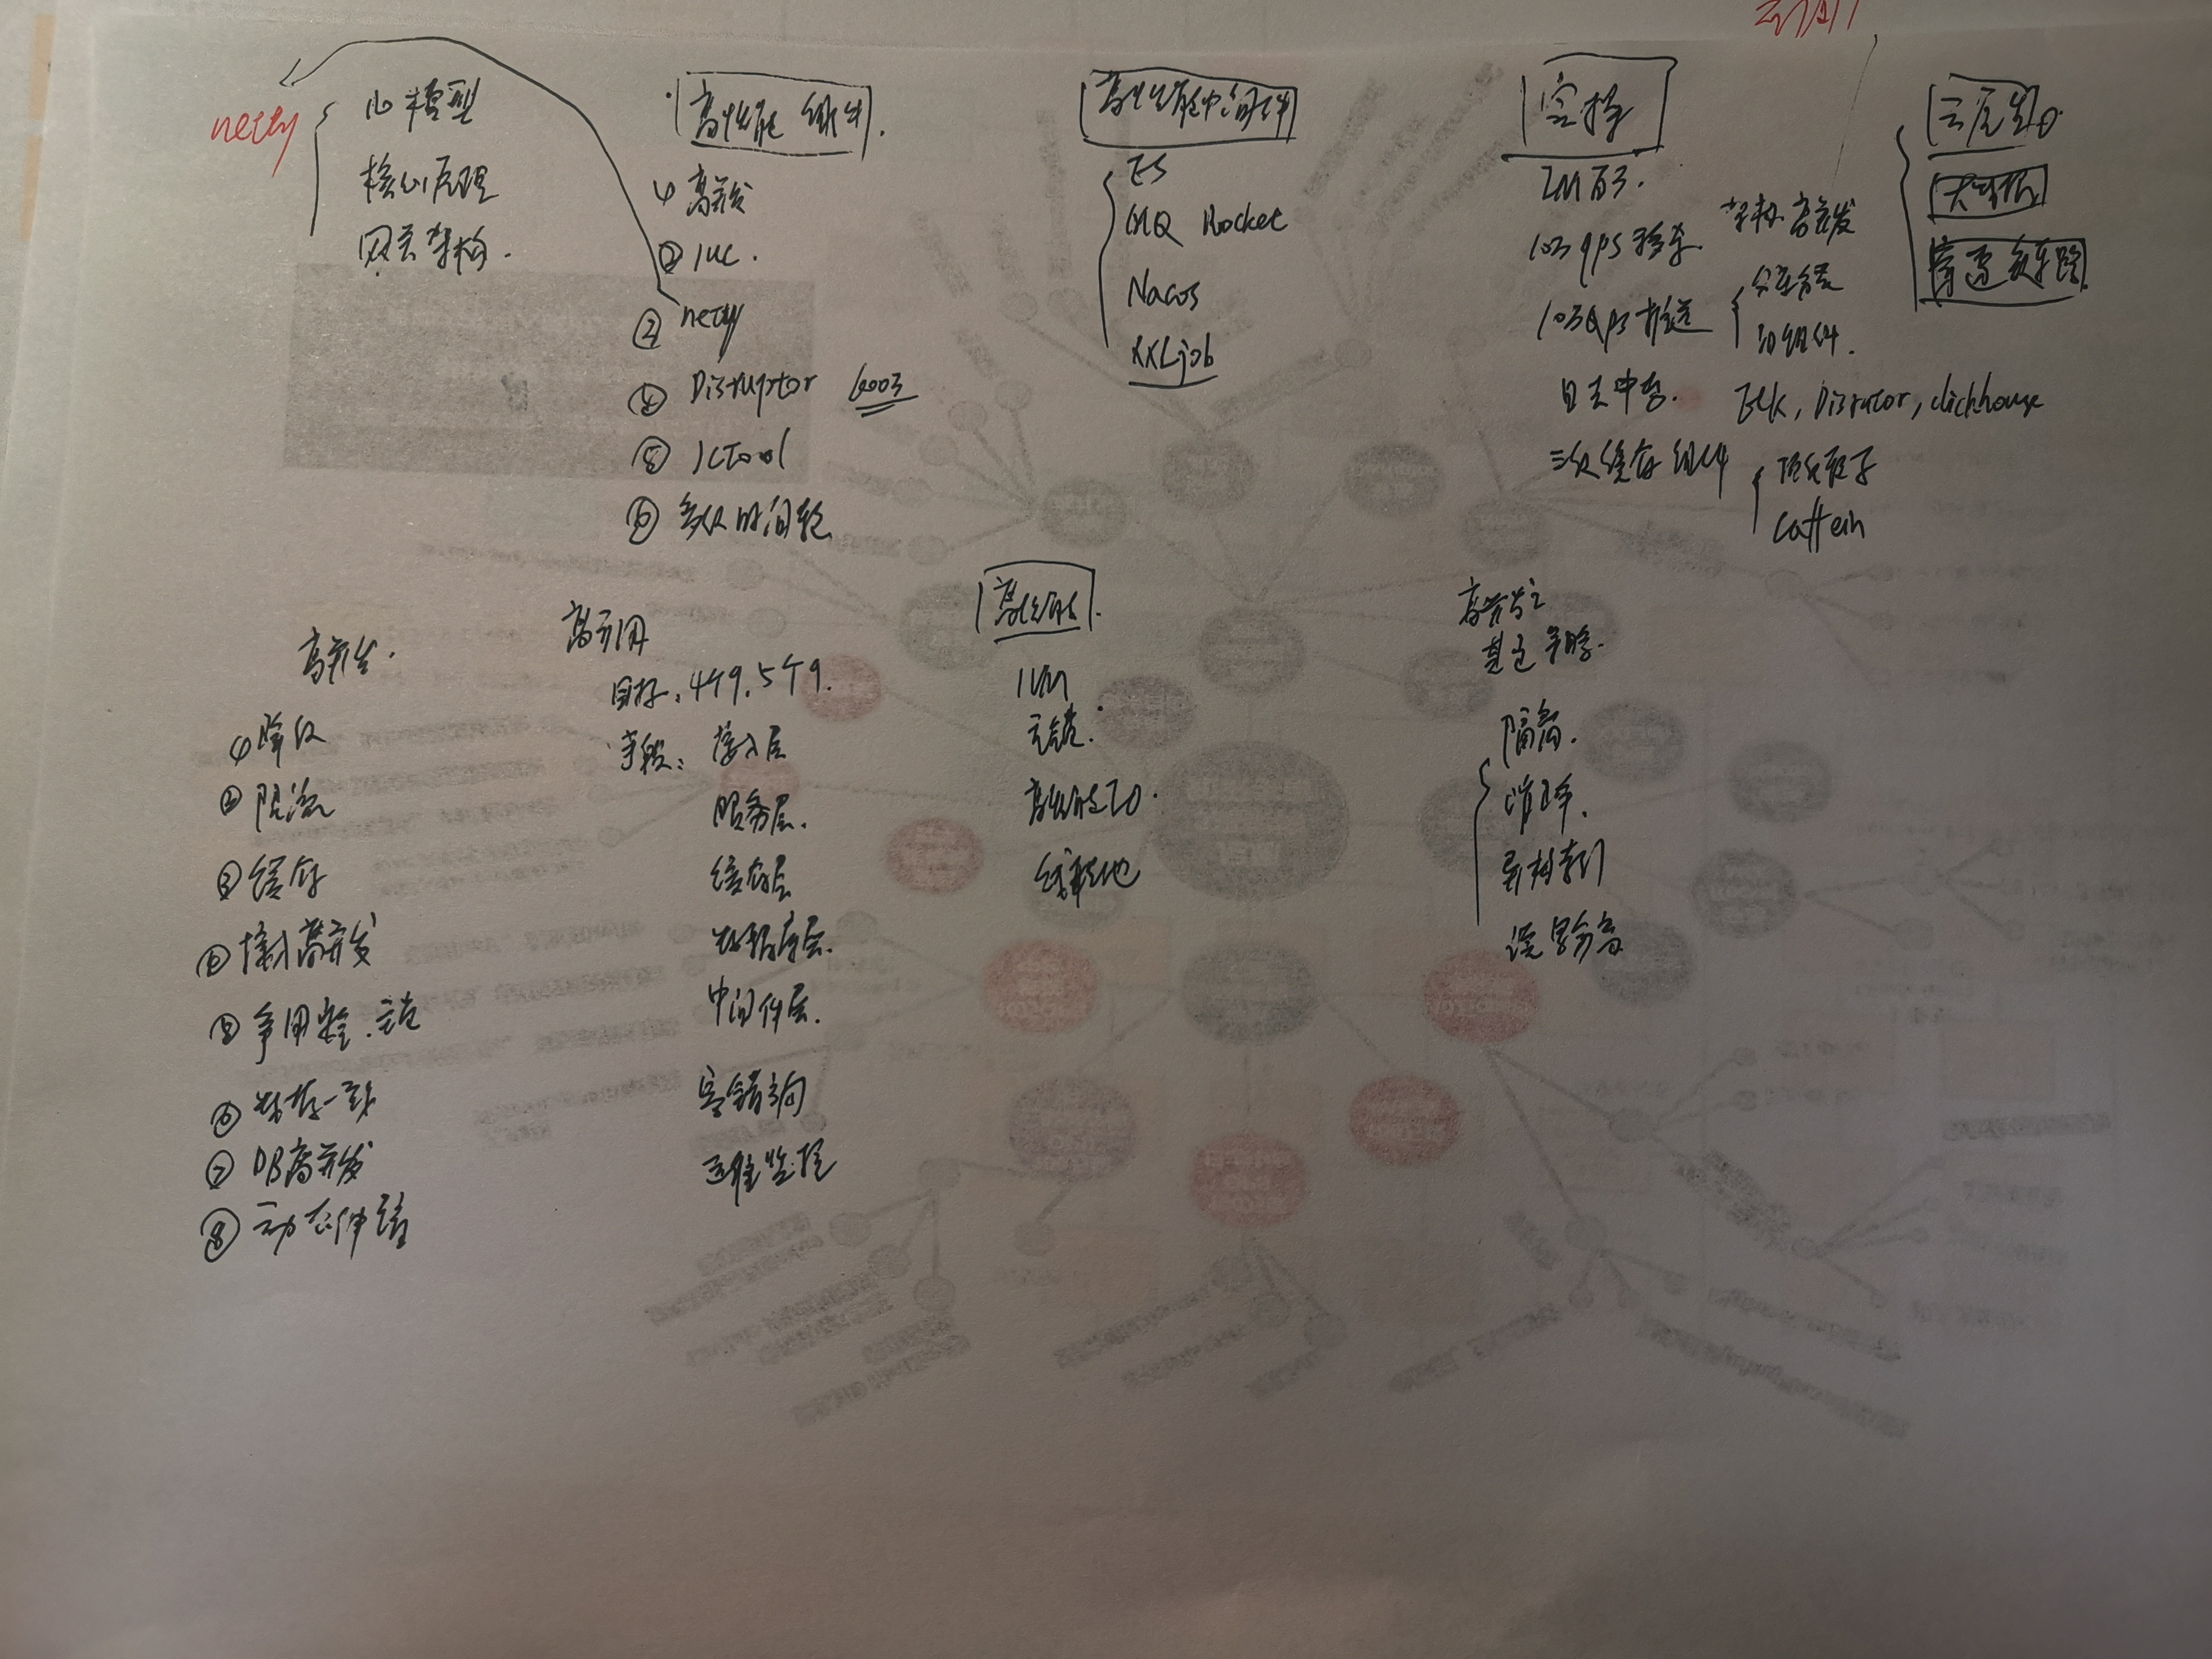
\includegraphics[width=1.1\textwidth]{images/nienjiagou2025.jpg} % 确保替换为你的图片路径
    %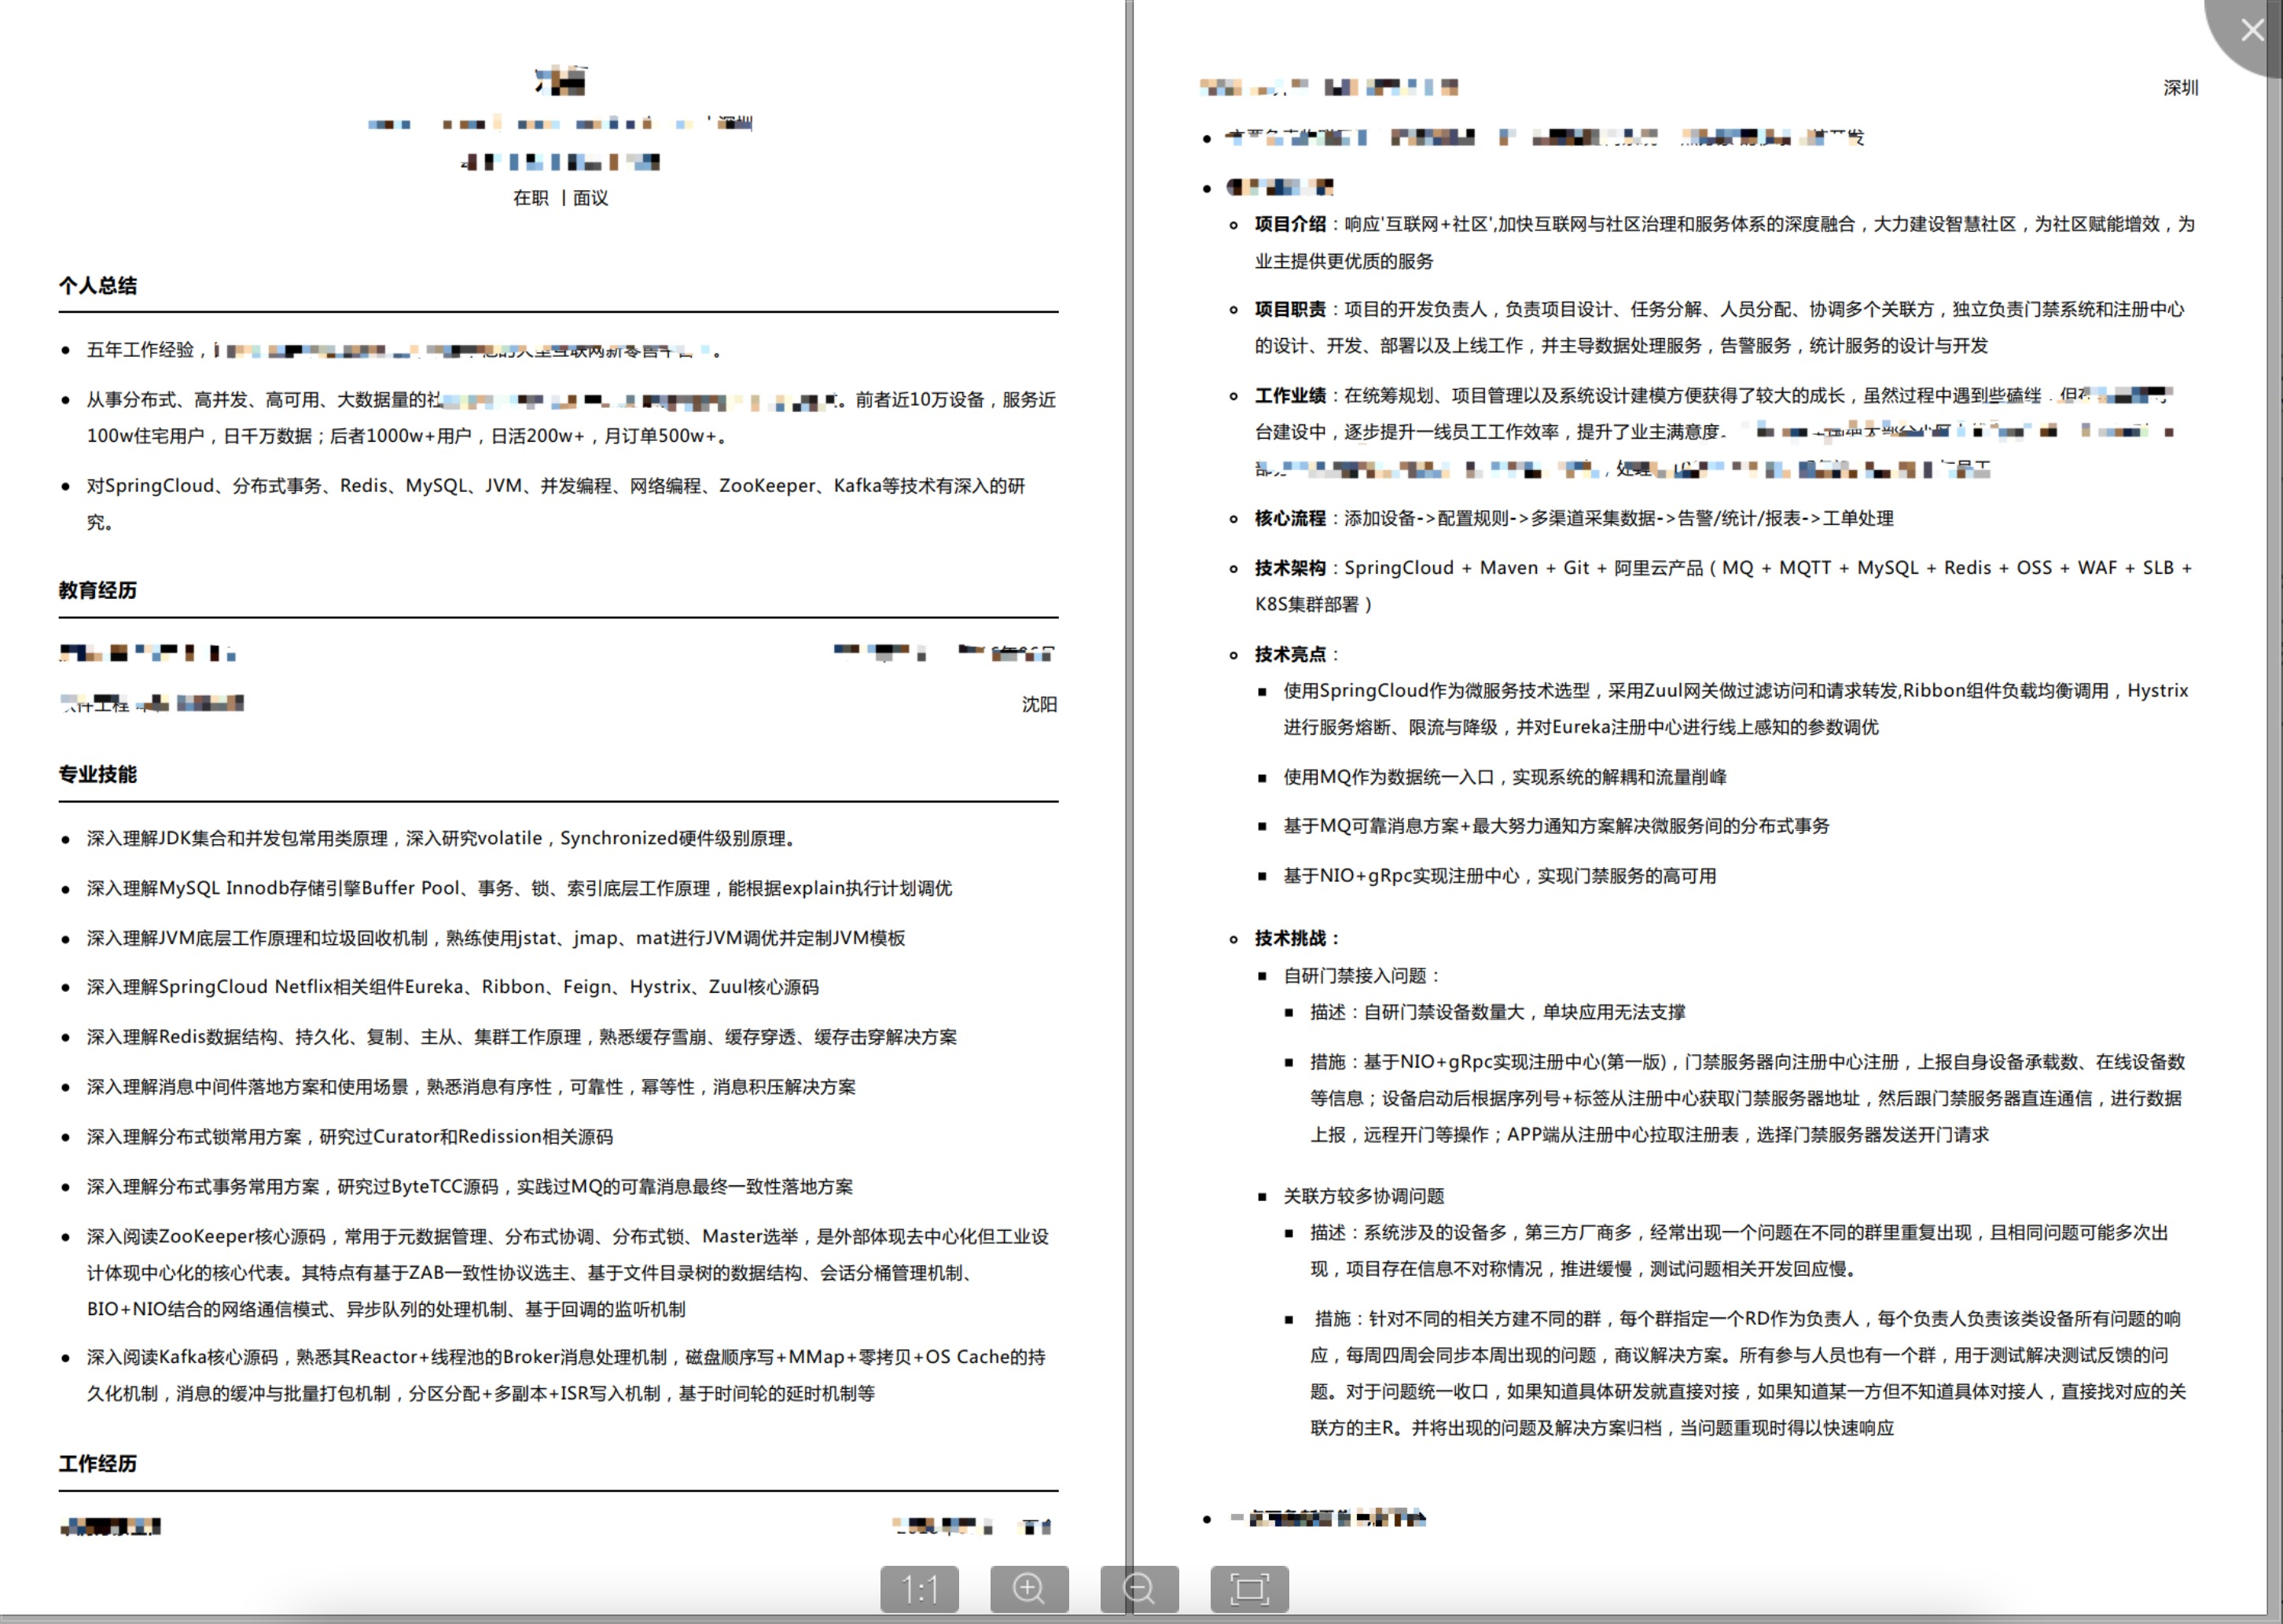
\includegraphics[width=\textwidth, height=\textheight]{resumes_ample.jpg} % 确保替换为你的图片路径    
  \end{sideways}
    \caption{nien架构}
    \label{fig:example}
  \end{figure}


\newpage
\section{nien}

第1章:9 史上最强线程池学习盛宴

第2章:6 Netty核心原理与底层知识学习盛宴

第3章:7 NettyByteBuf学习盛宴

第4章:3 百万级IM实战——CrazyIM会话管理

第5章:1 Java必备——Netty高并发灵魂编程

第6章:11 九阳真经:彻底揭秘NIO、Selector底层原理

第7章:2 底层解读:解密核心难题,秒杀外国权威

第8章:27 Netty大实战:从0到1开始亿级流量CrazyIM开发

第10章:11-10W QPS真刀实操以及基于ZK+Netty手写分布式测试工具

第11章. 4- 5分钟把简历变得闪闪发光,人见人爱,回头率100%

第12章.22-吊打面试官:彻底明白分布式事务原理,以及seata的AT、TCC原理与实操

第13章.21-史上最强:从0开始Netty IM 实战,40岁老架构师细致解读,实战之中处处透着原理和精髓

第14章.40-横扫全网,elasticsearch底层原理与高可用架构实操,40岁老架构师细致解读,处处透着原理和精髓

第15章:5-《springcloud nginx 高并发核心编程》配套视频

第16章:73-葵花宝典(高性能秘籍)

第17章:45-横扫全网系列:工业级rocketmq高可用底层原理和实操

第18章:80-架构师超级内功篇:rocketmq源码学习以及3高架构模式解读

第19.1章vep:61-10Wqps推送中台从架构到实操

第19章:35-10Wqps推送中台实操(下)

第20章:156-横扫全网系列:彻底穿透Netty原理与实操

第21章:19-6个面试必备 Redis cluster的核心实操

第22章:65-彻底穿透Netty架构与源码, 一卷到底,卷透底层

第23章sz:70-100W级别QPS日志平台实操

第24章sz:46-资深架构必备,彻底穿透Skywalking链路跟踪源码、JavaAgent探针技术

第25章sz:42-彻底穿透400W级OPS缓存之王Caffeine底层架构、核心源码

第26章sz:52-超高并发场景100Wqps三级缓存组件原理和实操

第27章sz:16-全链路异步超底层原理和实操:手写 hystrix 熔断 + webflux + Lettuce + Dubbo

第28章sz:30-穿透云原生K8S+Jenkins+SpringCloud底层原理和实操

第29章sz:61-Golang学习圣经,高并发Go+Java混合微服务架构与实操

第30章sz:6-Java调优圣经——顶尖高手的调优绝技

第31章sz:17-超高并发1000W级 golang 推送中台 架构与实操

第32章sz:19-超高并发、超高可用1000W级 ID组件 架构与实操

第33章sz:41-10Wqps高并发Netty网关架构与实操(1)

第34章, 30-DDD学习圣经,从未开始DDD架构和落地

第35章: 46-中间件塔尖实战—穿透Netty对象池、内存池

第36章:22-进大厂、做架构 顶奢核心面试题(第一期)

第37章: 25-百亿级数据存储架构:MYSQL双写 + HABSE +Flink +ES综合大实操

第38章:12-ElasticSearch 学习圣经:从0到1, 精通  ElasticSearch 工业级实操

第39章:12-XXl-JOB学习圣经:从0到1, 精通  xxl-job工业级实操

第40章:11-HBASE学习圣经:从0到1, 精通  HBASE的底层原理和实操

第41章:7-Flink学习圣经:从0到1, 精通 Flink 的底层原理和实操

第42-46章:尼恩Java硬核架构班4 微服务底座-讲义与源码

42-token      25

43-dubbo     20

44-nacos      17

45-sentinel  27
    
46-elk,felk 22


\newpage

\section{账号}

192.168.1.7

8.2账户
root/root123

用户:seeyon

密码统一:Jsyh@123

mysqldump -uroot -p seeyon > seeyon.sql

mysql -uroot -p seeyon82b < seeyon.sql


8.0账户
mysql

root/root123

ALTER USER 'root'@'localhost' IDENTIFIED WITH mysql\_native\_password BY 'root123';

system/system12

group-admin/groupadmin12

s1agent/s1agent12

seeyon/user123456

admin1/user123456

01011001/user123456

new-normal-user/user123456

\newpage

\end{document}
